\chapter{Resultados}
Neste capítulo serão descritos os resultados obtidos através da simulação da
EDP com a variação de diversos parâmetros. Os parâmetros iniciais escolhidos
para este trabalho foram:
\begin{itemize}
    \item $L_x = 10$m (comprimento do domínio)
    \item $nx = 200$ (número de células)
    \item $\bar{u} = 2$m/s (velocidade de escoamento)
    \item $t_\text{final} = 1$s  (tempo final de simulação)
    \item $\Delta t = 0,9\left( \frac{\Delta_x}{\bar{u}} \right) = 0,0225$
    (passo de tempo)
    \item $A = 100$
    \item $B = 1,5$
    \item $C = 4,0$
    \item $D = 6,0$
    \item $E = 2,0$
\end{itemize}

\section{Forward Time-Backward Space (FTBS)}

\subsection{Resultados para variações de $nx$}
Com a variação de $nx$, obtiveram-se os seguintes resultados:
\begin{figure}[H]
    \centering
    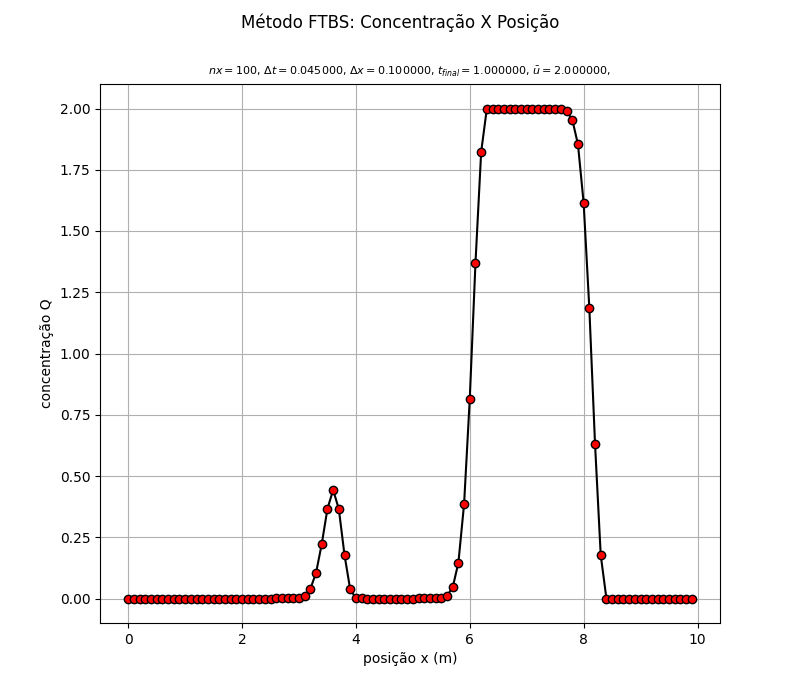
\includegraphics[width=0.7\textwidth]{FTBSnx100}
    \caption{$nx = 100$}
\end{figure}
\begin{figure}[H]
    \centering
    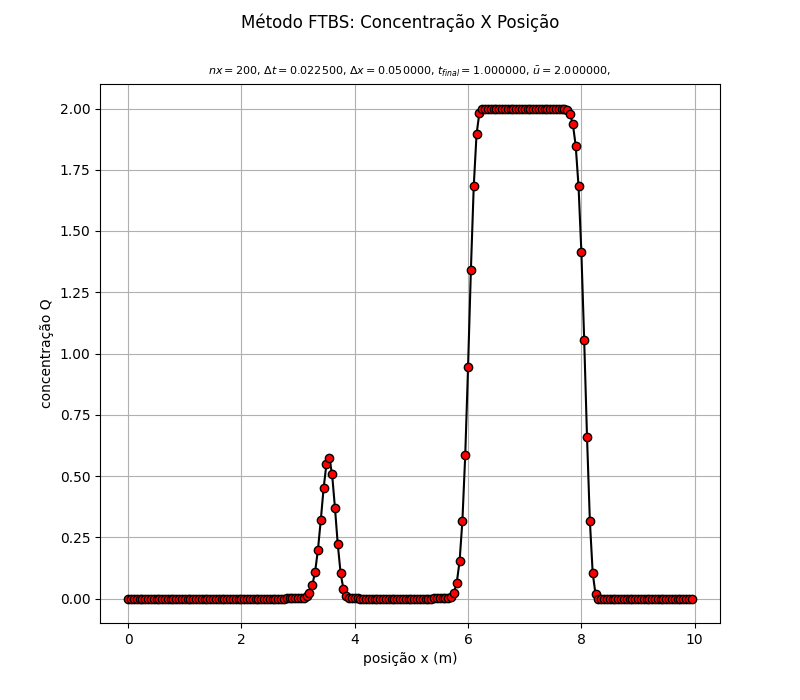
\includegraphics[width=0.7\textwidth]{FTBSnx200}
    \caption{$nx = 200$m}
\end{figure}
\begin{figure}[H]
    \centering
    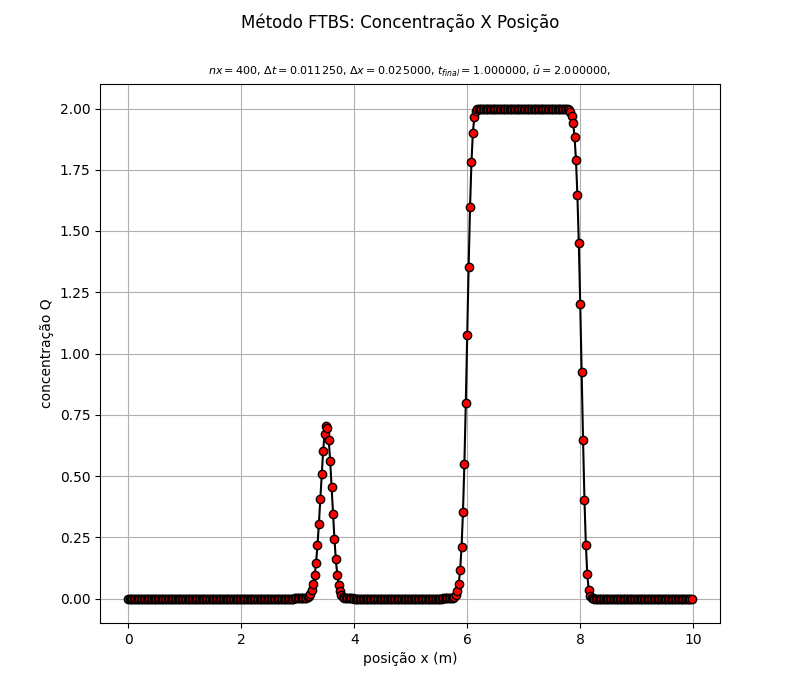
\includegraphics[width=0.7\textwidth]{FTBSnx400}
    \caption{$nx = 400$m}
\end{figure}
<inserir observações>

\subsection{Resultados para variações de $t_{\text{final}}$}
Com a variação de $t_{\text{final}}$, obtiveram-se os seguintes resultados:
\begin{figure}[H]
    \centering
    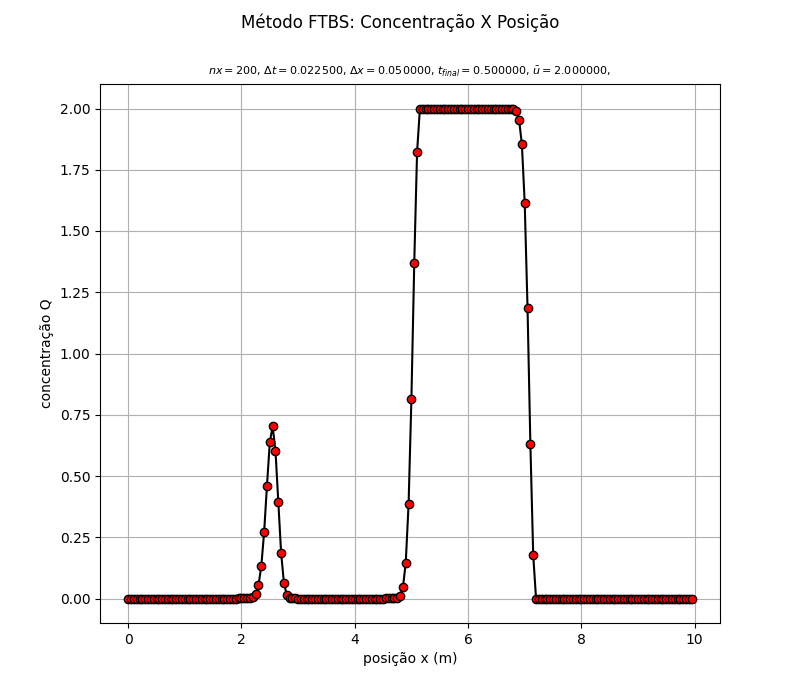
\includegraphics[width=0.7\textwidth]{FTBSt_final0,5}
    \caption{$t_{\text{final}} = 0,5$s}
\end{figure}
\begin{figure}[H]
    \centering
    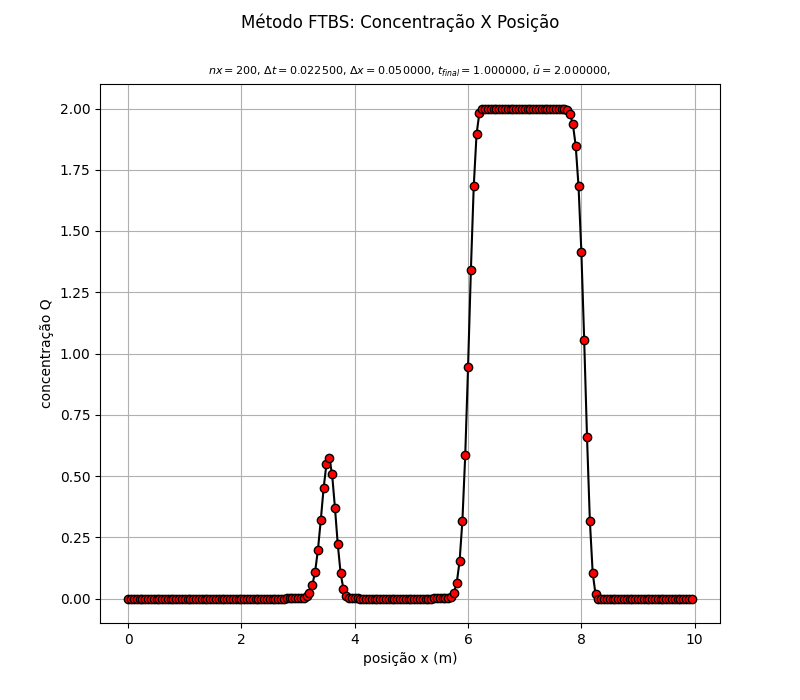
\includegraphics[width=0.7\textwidth]{FTBSt_final1,0}
    \caption{$t_{\text{final}} = 1,0$s}
\end{figure}
\begin{figure}[H]
    \centering
    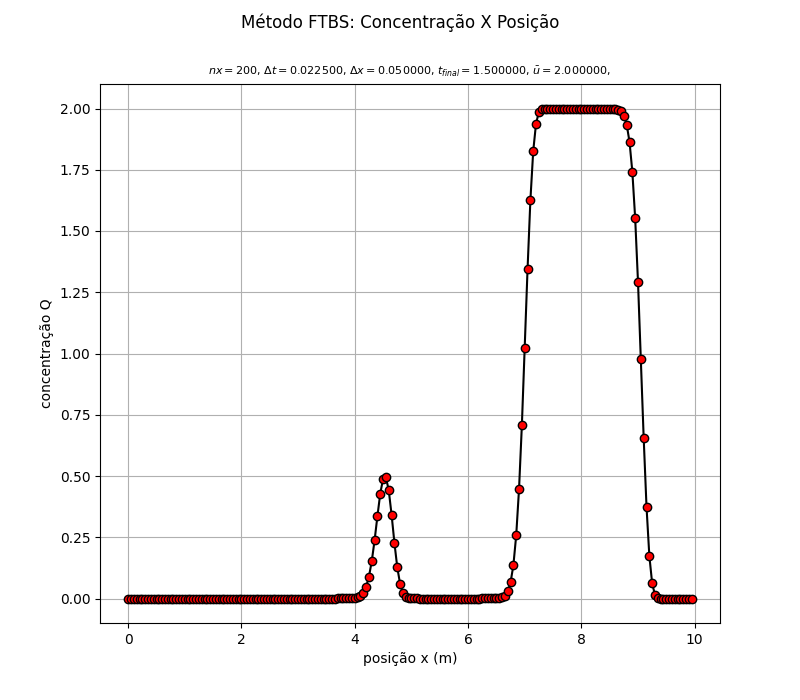
\includegraphics[width=0.7\textwidth]{FTBSt_final1,5}
    \caption{$t_{\text{final}} = 1,5$s}
\end{figure}
<inserir observações>

\section{Lax-Friedrichs (L-F)}

\subsection{Resultados para variações de $nx$}
Com a variação de $nx$, obtiveram-se os seguintes resultados:
\begin{figure}[H]
    \centering
    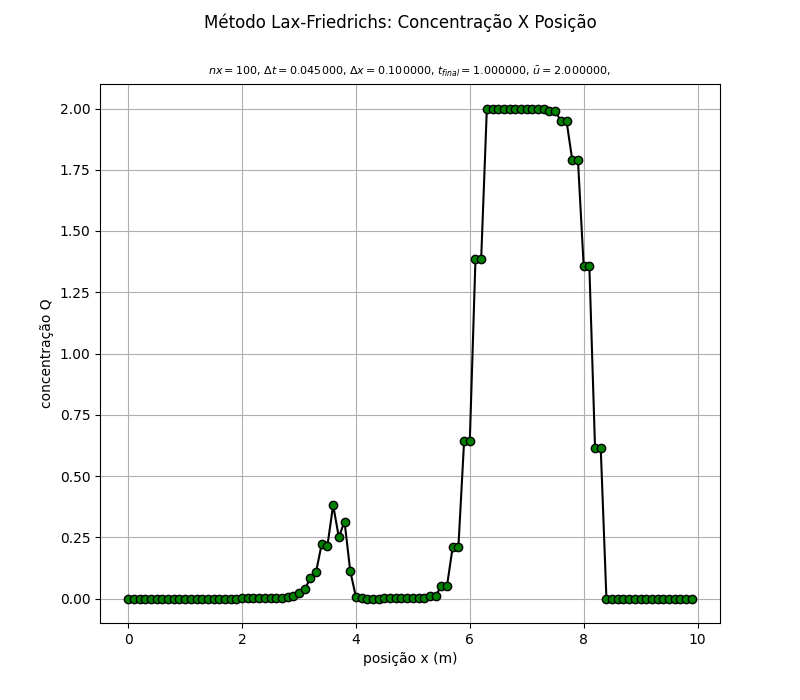
\includegraphics[width=0.7\textwidth]{LFnx100}
    \caption{$nx = 100$}
\end{figure}
\begin{figure}[H]
    \centering
    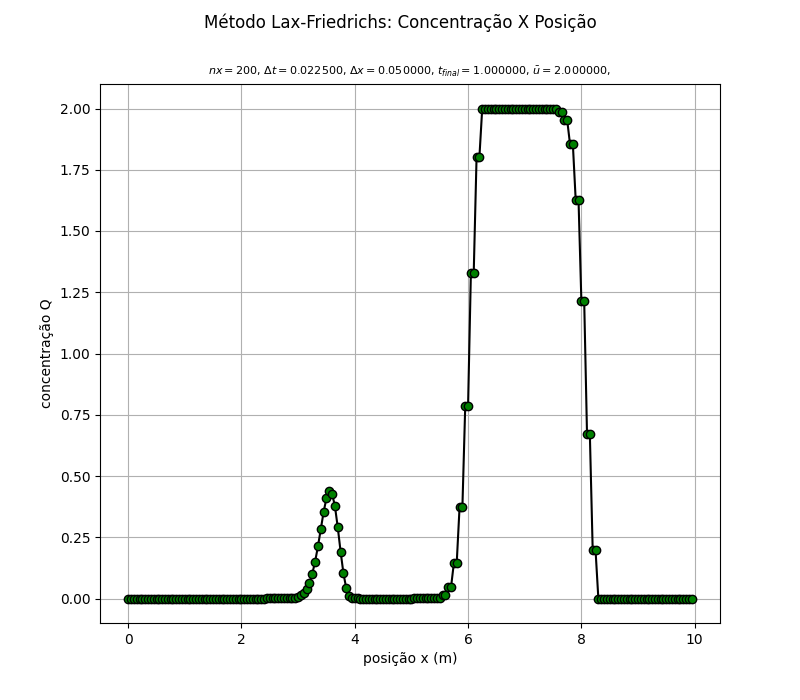
\includegraphics[width=0.7\textwidth]{LFnx200}
    \caption{$nx = 200$m}
\end{figure}
\begin{figure}[H]
    \centering
    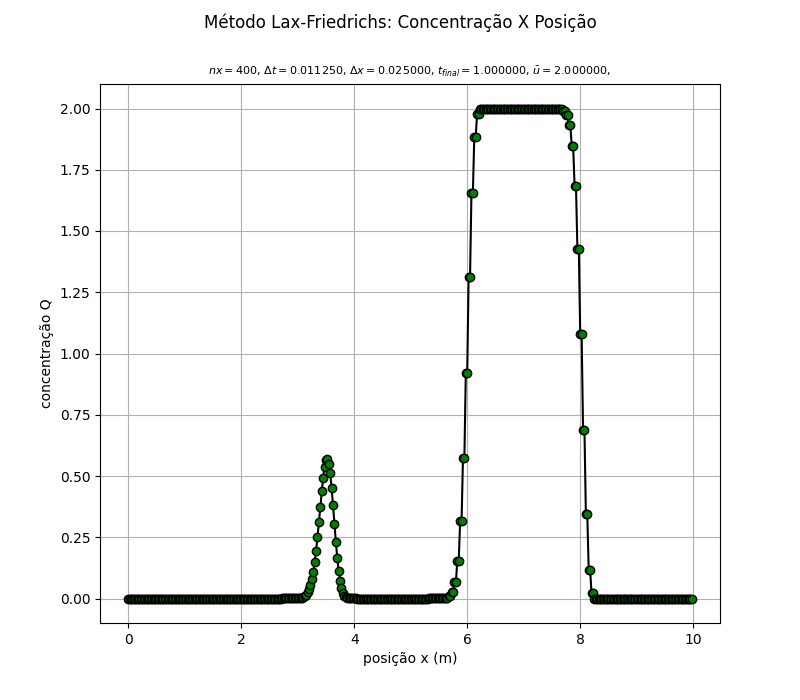
\includegraphics[width=0.7\textwidth]{LFnx400}
    \caption{$nx = 400$m}
\end{figure}
<inserir observações>

\subsection{Resultados para variações de $t_{\text{final}}$}
Com a variação de $t_{\text{final}}$, obtiveram-se os seguintes resultados:
\begin{figure}[H]
    \centering
    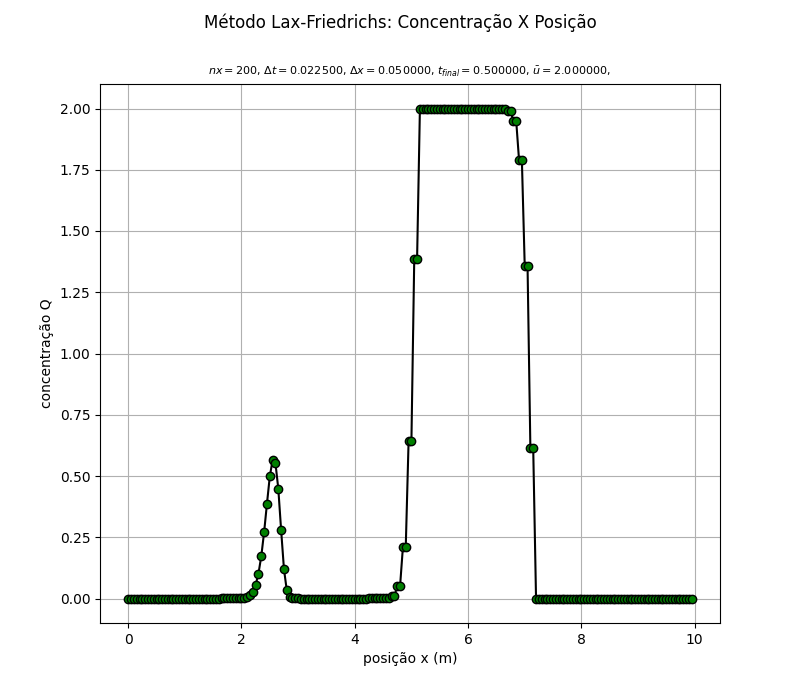
\includegraphics[width=0.7\textwidth]{LFt_final0,5}
    \caption{$t_{\text{final}} = 0,5$s}
\end{figure}
\begin{figure}[H]
    \centering
    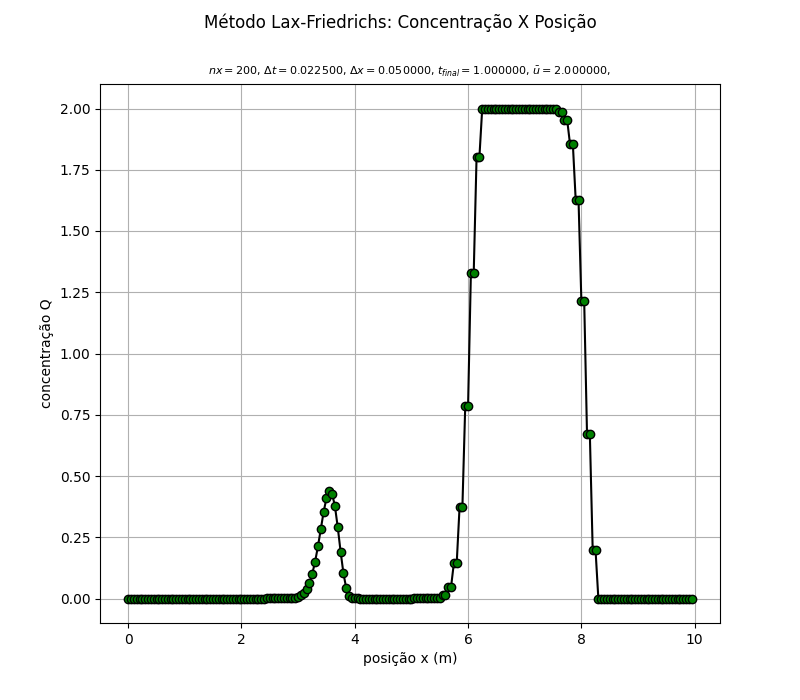
\includegraphics[width=0.7\textwidth]{LFt_final1,0}
    \caption{$t_{\text{final}} = 1,0$s}
\end{figure}
\begin{figure}[H]
    \centering
    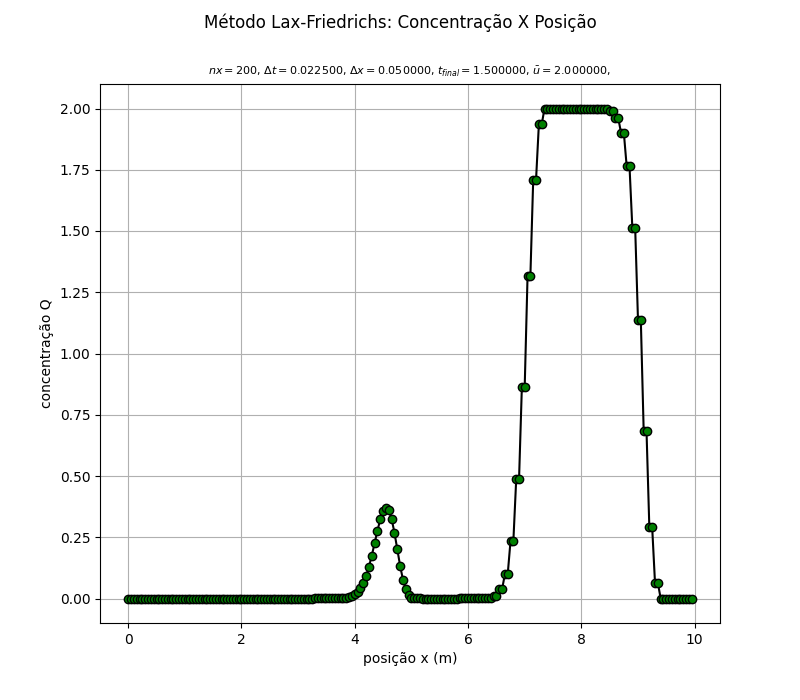
\includegraphics[width=0.7\textwidth]{LFt_final1,5}
    \caption{$t_{\text{final}} = 1,5$s}
\end{figure}
<inserir observações>

\section{Lax-Wendroff (L-W)}

\subsection{Resultados para variações de $nx$}
Com a variação de $nx$, obtiveram-se os seguintes resultados:
\begin{figure}[H]
    \centering
    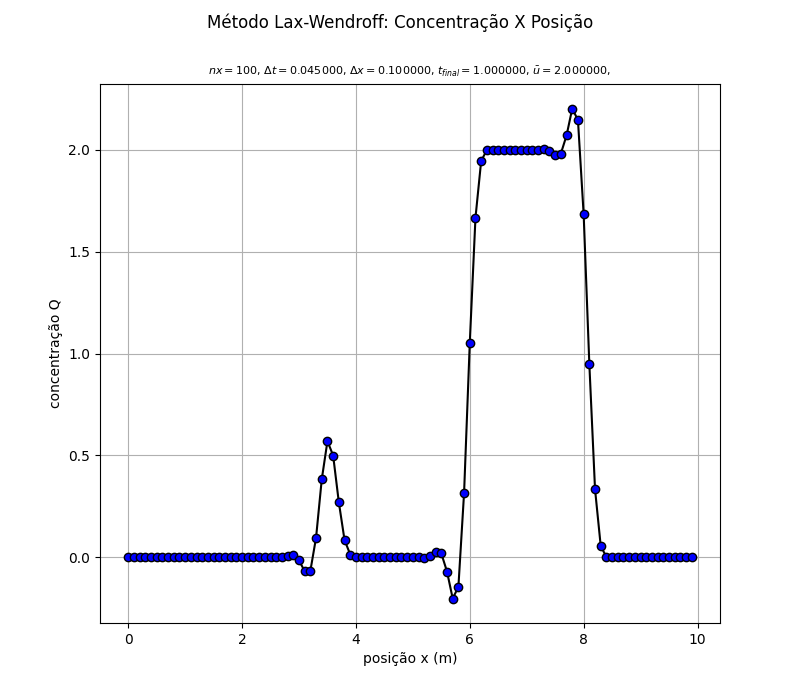
\includegraphics[width=0.7\textwidth]{LWnx100}
    \caption{$nx = 100$}
\end{figure}
\begin{figure}[H]
    \centering
    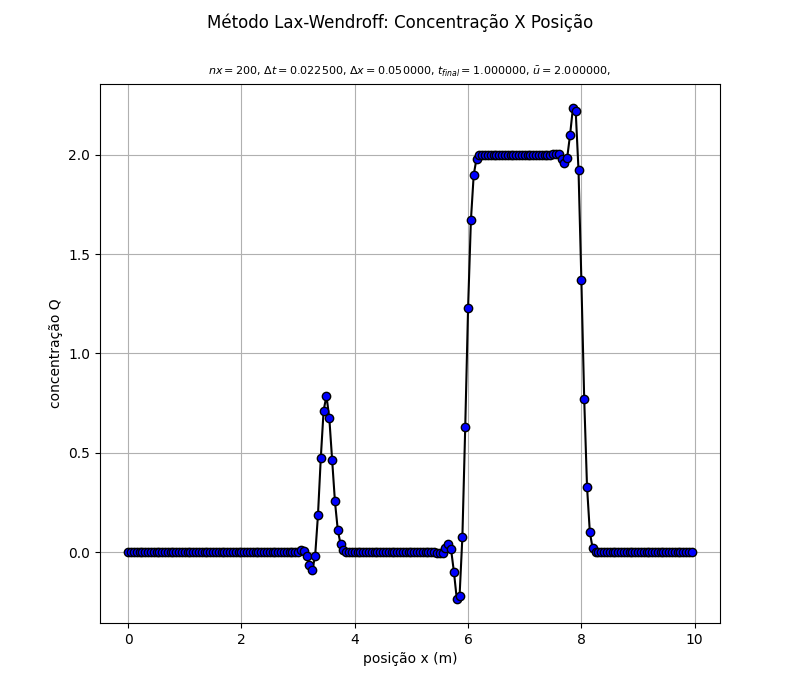
\includegraphics[width=0.7\textwidth]{LWnx200}
    \caption{$nx = 200$m}
\end{figure}
\begin{figure}[H]
    \centering
    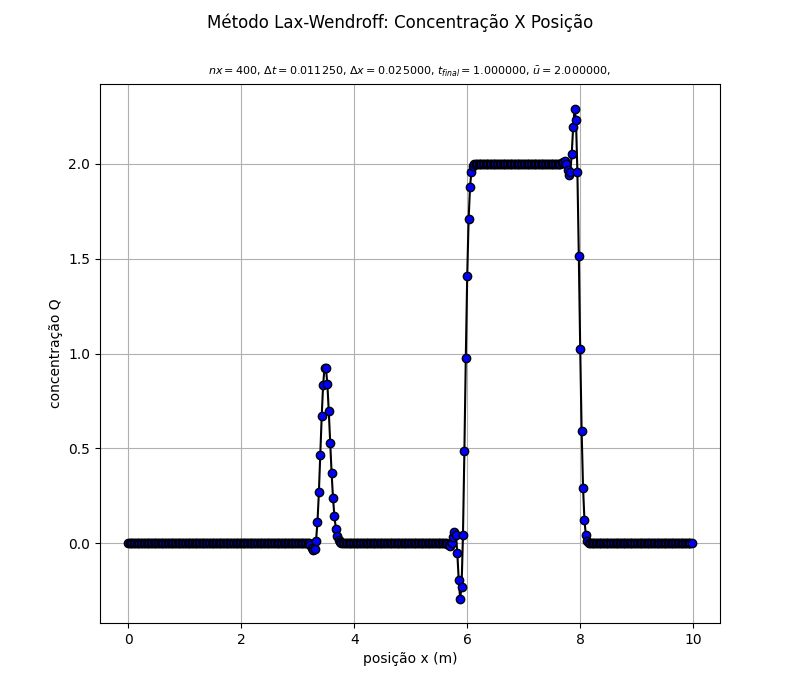
\includegraphics[width=0.7\textwidth]{LWnx400}
    \caption{$nx = 400$m}
\end{figure}
<inserir observações>

\subsection{Resultados para variações de $t_{\text{final}}$}
Com a variação de $t_{\text{final}}$, obtiveram-se os seguintes resultados:
\begin{figure}[H]
    \centering
    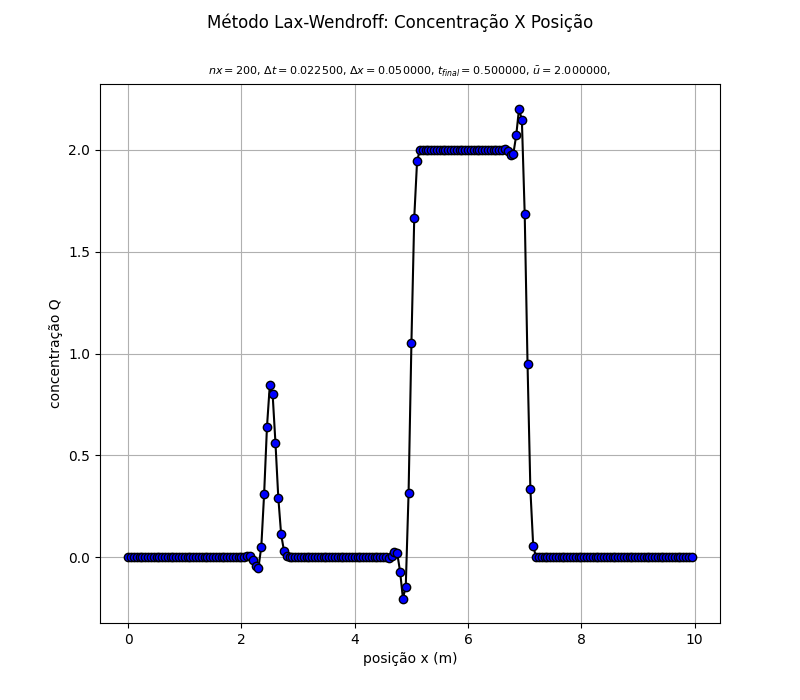
\includegraphics[width=0.7\textwidth]{LWt_final0,5}
    \caption{$t_{\text{final}} = 0,5$s}
\end{figure}
\begin{figure}[H]
    \centering
    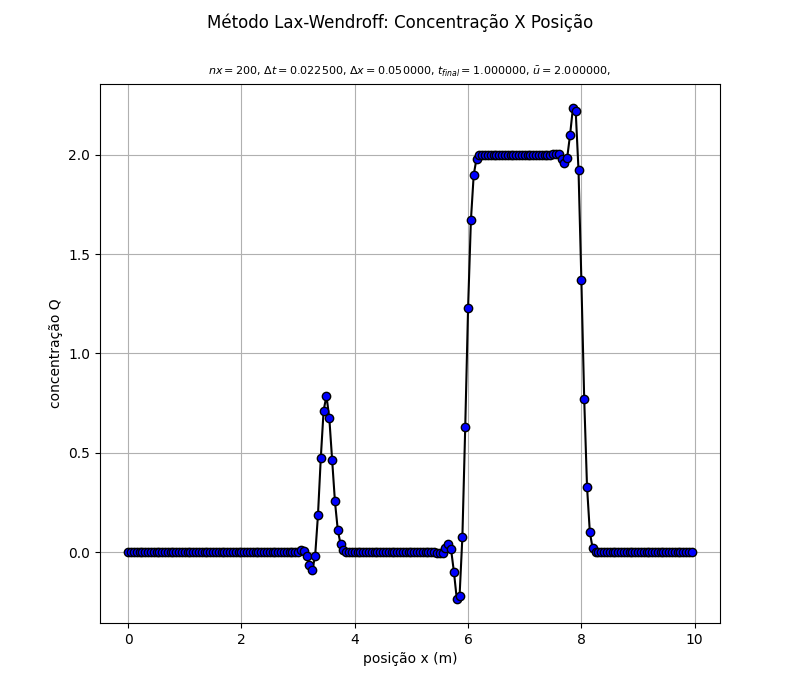
\includegraphics[width=0.7\textwidth]{LWt_final1,0}
    \caption{$t_{\text{final}} = 1,0$s}
\end{figure}
\begin{figure}[H]
    \centering
    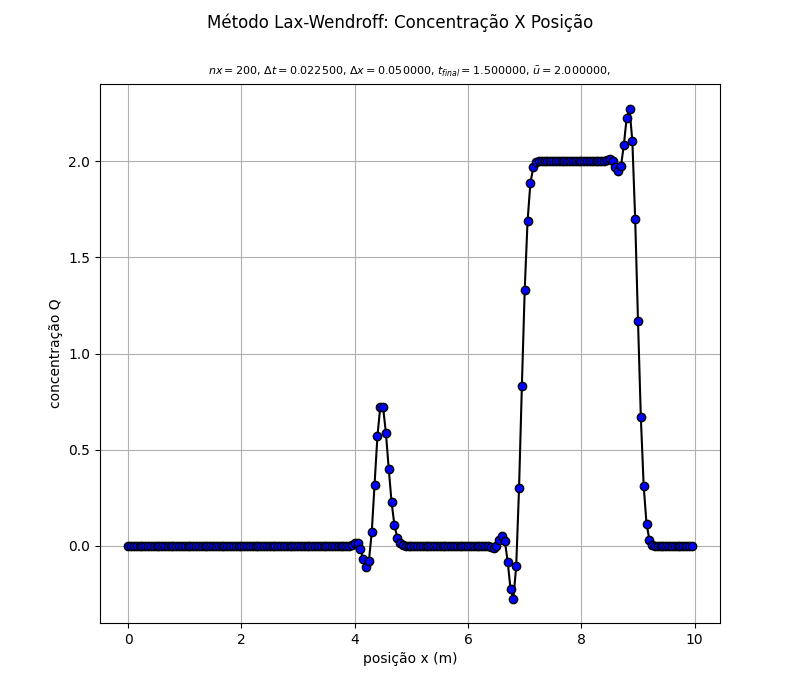
\includegraphics[width=0.7\textwidth]{LWt_final1,5}
    \caption{$t_{\text{final}} = 1,5$s}
\end{figure}
<inserir observações>

\section{Beam-Warming (B-W)}

\subsection{Resultados para variações de $nx$}
Com a variação de $nx$, obtiveram-se os seguintes resultados:
\begin{figure}[H]
    \centering
    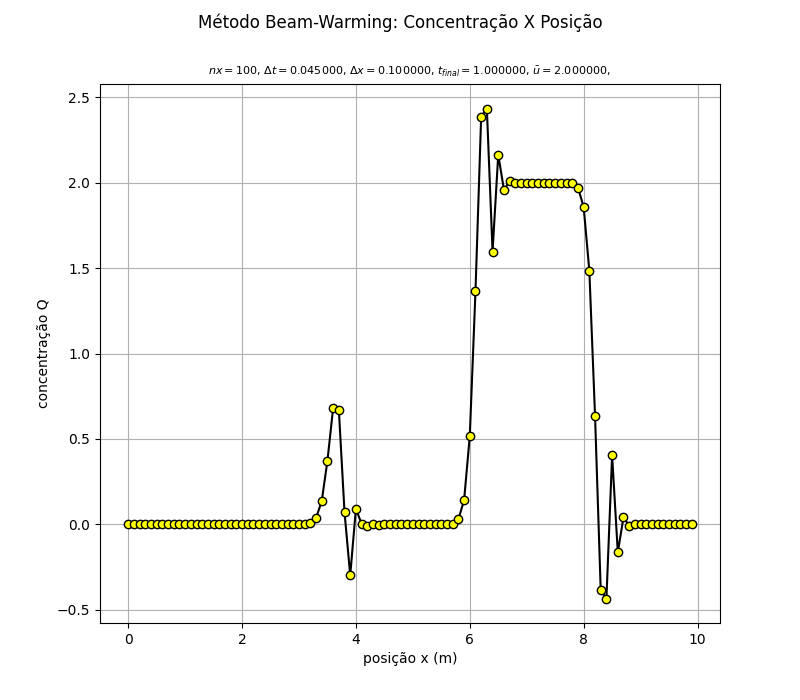
\includegraphics[width=0.7\textwidth]{BWnx100}
    \caption{$nx = 100$}
\end{figure}
\begin{figure}[H]
    \centering
    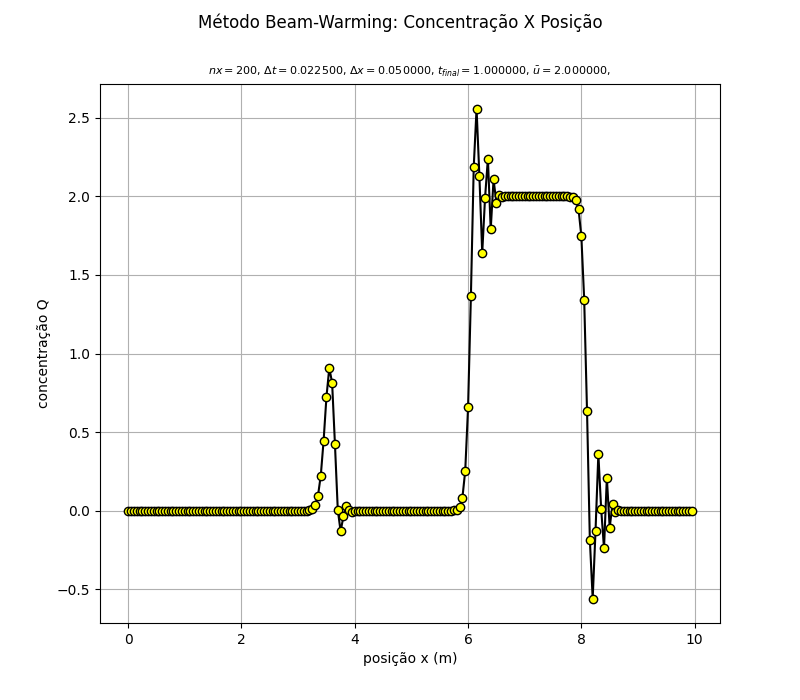
\includegraphics[width=0.7\textwidth]{BWnx200}
    \caption{$nx = 200$m}
\end{figure}
\begin{figure}[H]
    \centering
    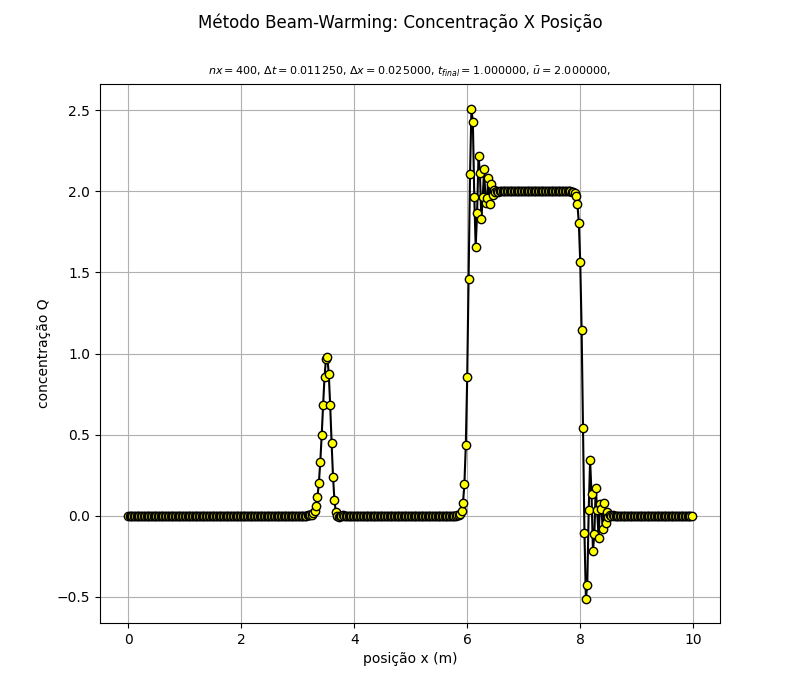
\includegraphics[width=0.7\textwidth]{BWnx400}
    \caption{$nx = 400$m}
\end{figure}
<inserir observações>

\subsection{Resultados para variações de $t_{\text{final}}$}
Com a variação de $t_{\text{final}}$, obtiveram-se os seguintes resultados:
\begin{figure}[H]
    \centering
    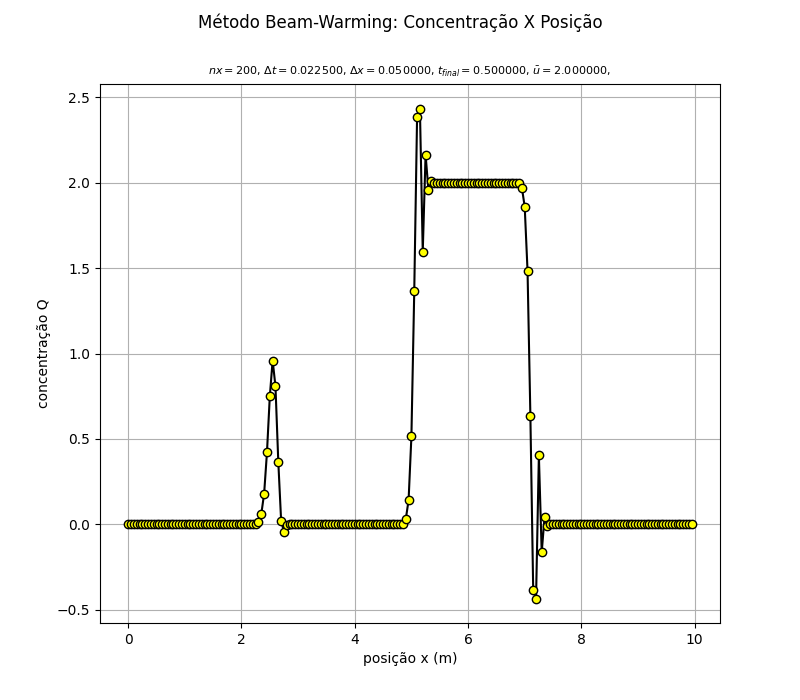
\includegraphics[width=0.7\textwidth]{BWt_final0,5}
    \caption{$t_{\text{final}} = 0,5$s}
\end{figure}
\begin{figure}[H]
    \centering
    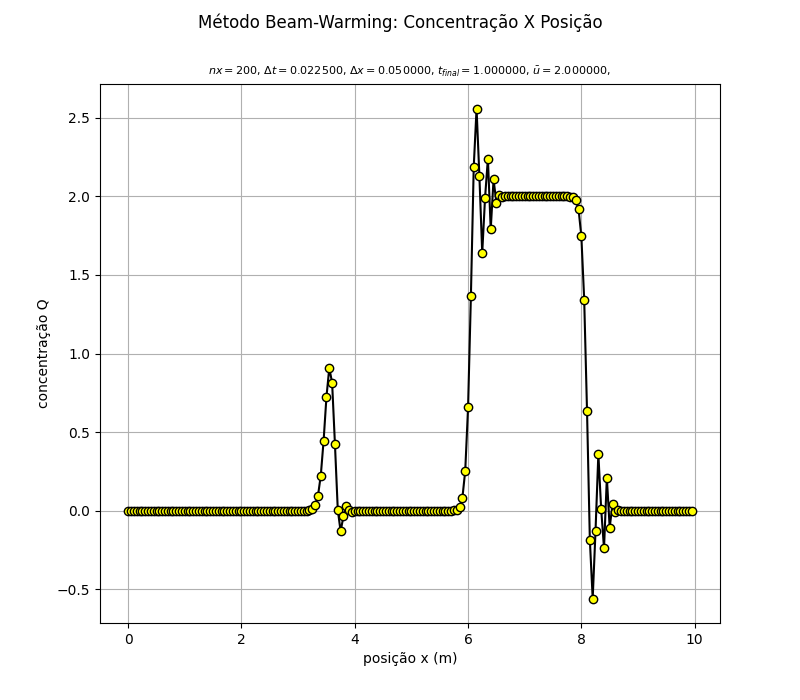
\includegraphics[width=0.7\textwidth]{BWt_final1,0}
    \caption{$t_{\text{final}} = 1,0$s}
\end{figure}
\begin{figure}[H]
    \centering
    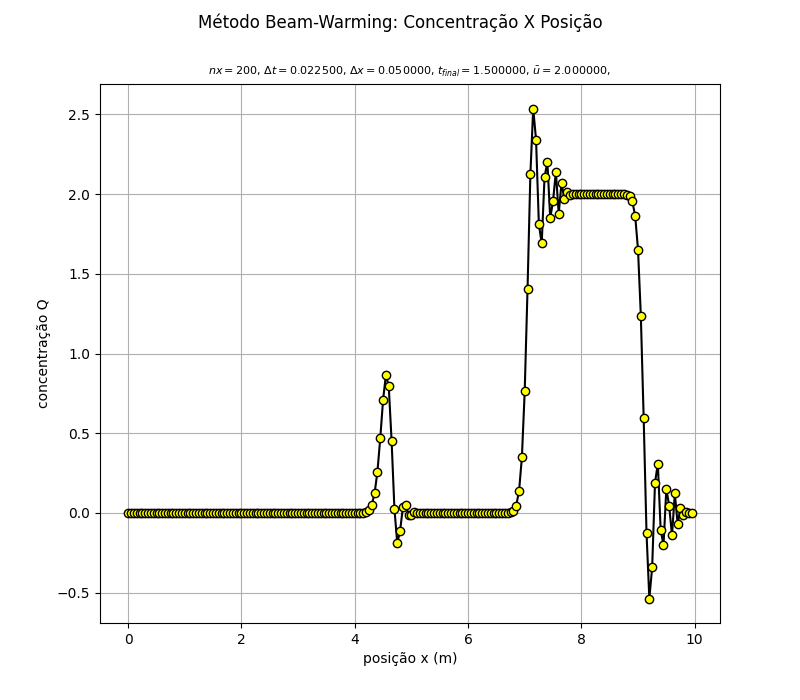
\includegraphics[width=0.7\textwidth]{BWt_final1,5}
    \caption{$t_{\text{final}} = 1,5$s}
\end{figure}
<inserir observações>